\subsection{Optimization Starting from a Circle}
\label{ch5:sec:cs1}

We first study the case of a 2D circle , which we aim to optimize to minimize drag, with the expectation that it will naturally converge toward the shape of a supercritical airfoil. This case involves significant geometric deformations, testing DeepGeo’s ability to maintain global shape smoothness while allowing large deformation freedom and ensuring robust mesh deformation under challenging conditions.

\subsubsection{Problem Formulation}

We begin with a 2D circle of diameter one and apply the same experimental setup as in the ADODG-2 transonic airfoil optimization benchmark~\footnote{\url{https://sites.google.com/view/mcgill-computational-aerogroup/adodg}}. The objective is to minimize the drag coefficient $C_D$ while maintaining the lift coefficient $C_L$ at $0.824$ and constraining the pitching moment coefficient to $C_M \geq -0.092$. The optimization is performed in a transonic turbulent flow with a Mach number of $0.734$, a Reynolds number of $5\times 10^6$ and an initial angle of attack of $2.0^{\circ}$. 
We used pyHyp~\cite{aa.Secco2021} to compute the CFD template mesh shown in Fig.~\ref{ch5:fig:cs1_template_mesh}(a), which comprises $20,331$ cells.

\begin{table}[htb]
  \centering
  \caption{\small Aerodynamic shape optimization task specifications for the Case Study I.}
  \resizebox{0.95\columnwidth}{!} {
        \begin{tabular}{lllrr}
        \hline
        \multicolumn{1}{l}{\textbf{Objectives}} & \textbf{Functions/Variables} & \textbf{Description} & \multicolumn{1}{l}{\textbf{DeepGeo Quantity}} & \multicolumn{1}{l}{\textbf{FFD Quantity}} \\
        \hline
        \multicolumn{1}{l}{\textbf{Minimize}} & $C_D$  & Drag coefficient &        &  \\
        \hline
        \multicolumn{1}{l}{\multirow{3}[2]{*}{\textbf{With respect to}}} & $\Theta$ & Weights of DeepGeo & \num{151585} &         \\
        \multicolumn{1}{l}{} & $P_z$  & Control points' $z$ coordinates &        & 30 \\
        \multicolumn{1}{l}{} & $\alpha$ & Angle of attack & 1      & 1 \\
        \hline
        \multicolumn{3}{l}{\textbf{Total design variables}} & \num{151586} & 31 \\
        \hline
        \multicolumn{1}{l}{\multirow{6}[2]{*}{\textbf{Subject to}}} & $C_L=0.824$ & Lift coefficient constraint & 1      & 1 \\
        \multicolumn{1}{r}{} & $C_M\leq0.092$ & Moment coefficient constraint & 1      & 1 \\
        \multicolumn{1}{r}{} & $t \ge 0.2\,t_\text{RAE2822}$ & Minimum thickness constraints &        & 30 \\
        \multicolumn{1}{r}{} & $A \ge 0.0654$ & Minimum area constraints &   1    &  1 \\
        \multicolumn{1}{r}{} & $\delta \bv^\text{TE}=0$ & Trailing edge constraint & 1      &  \\
        \multicolumn{1}{r}{} & $\delta \bv^\text{LE}=0$ & Leading edge constraint & 1      &  \\
        \multicolumn{1}{r}{} & $0.5 \leq \alpha \leq 4.0$ & Angle of attack constraint & 1      &  1 \\
        \hline
        \multicolumn{3}{l}{\textbf{Total constraints}} & 6      & 34 \\
        \hline
        \multicolumn{3}{l}{\textbf{Need value range limits for each DV?}} & NO     & YES \\
        \hline
        \end{tabular}%
    }
  \label{ch5:tab:circle_2_airfoil_DV_cons}%
\end{table}%

\begin{figure}[htb]
    \begin{center}
        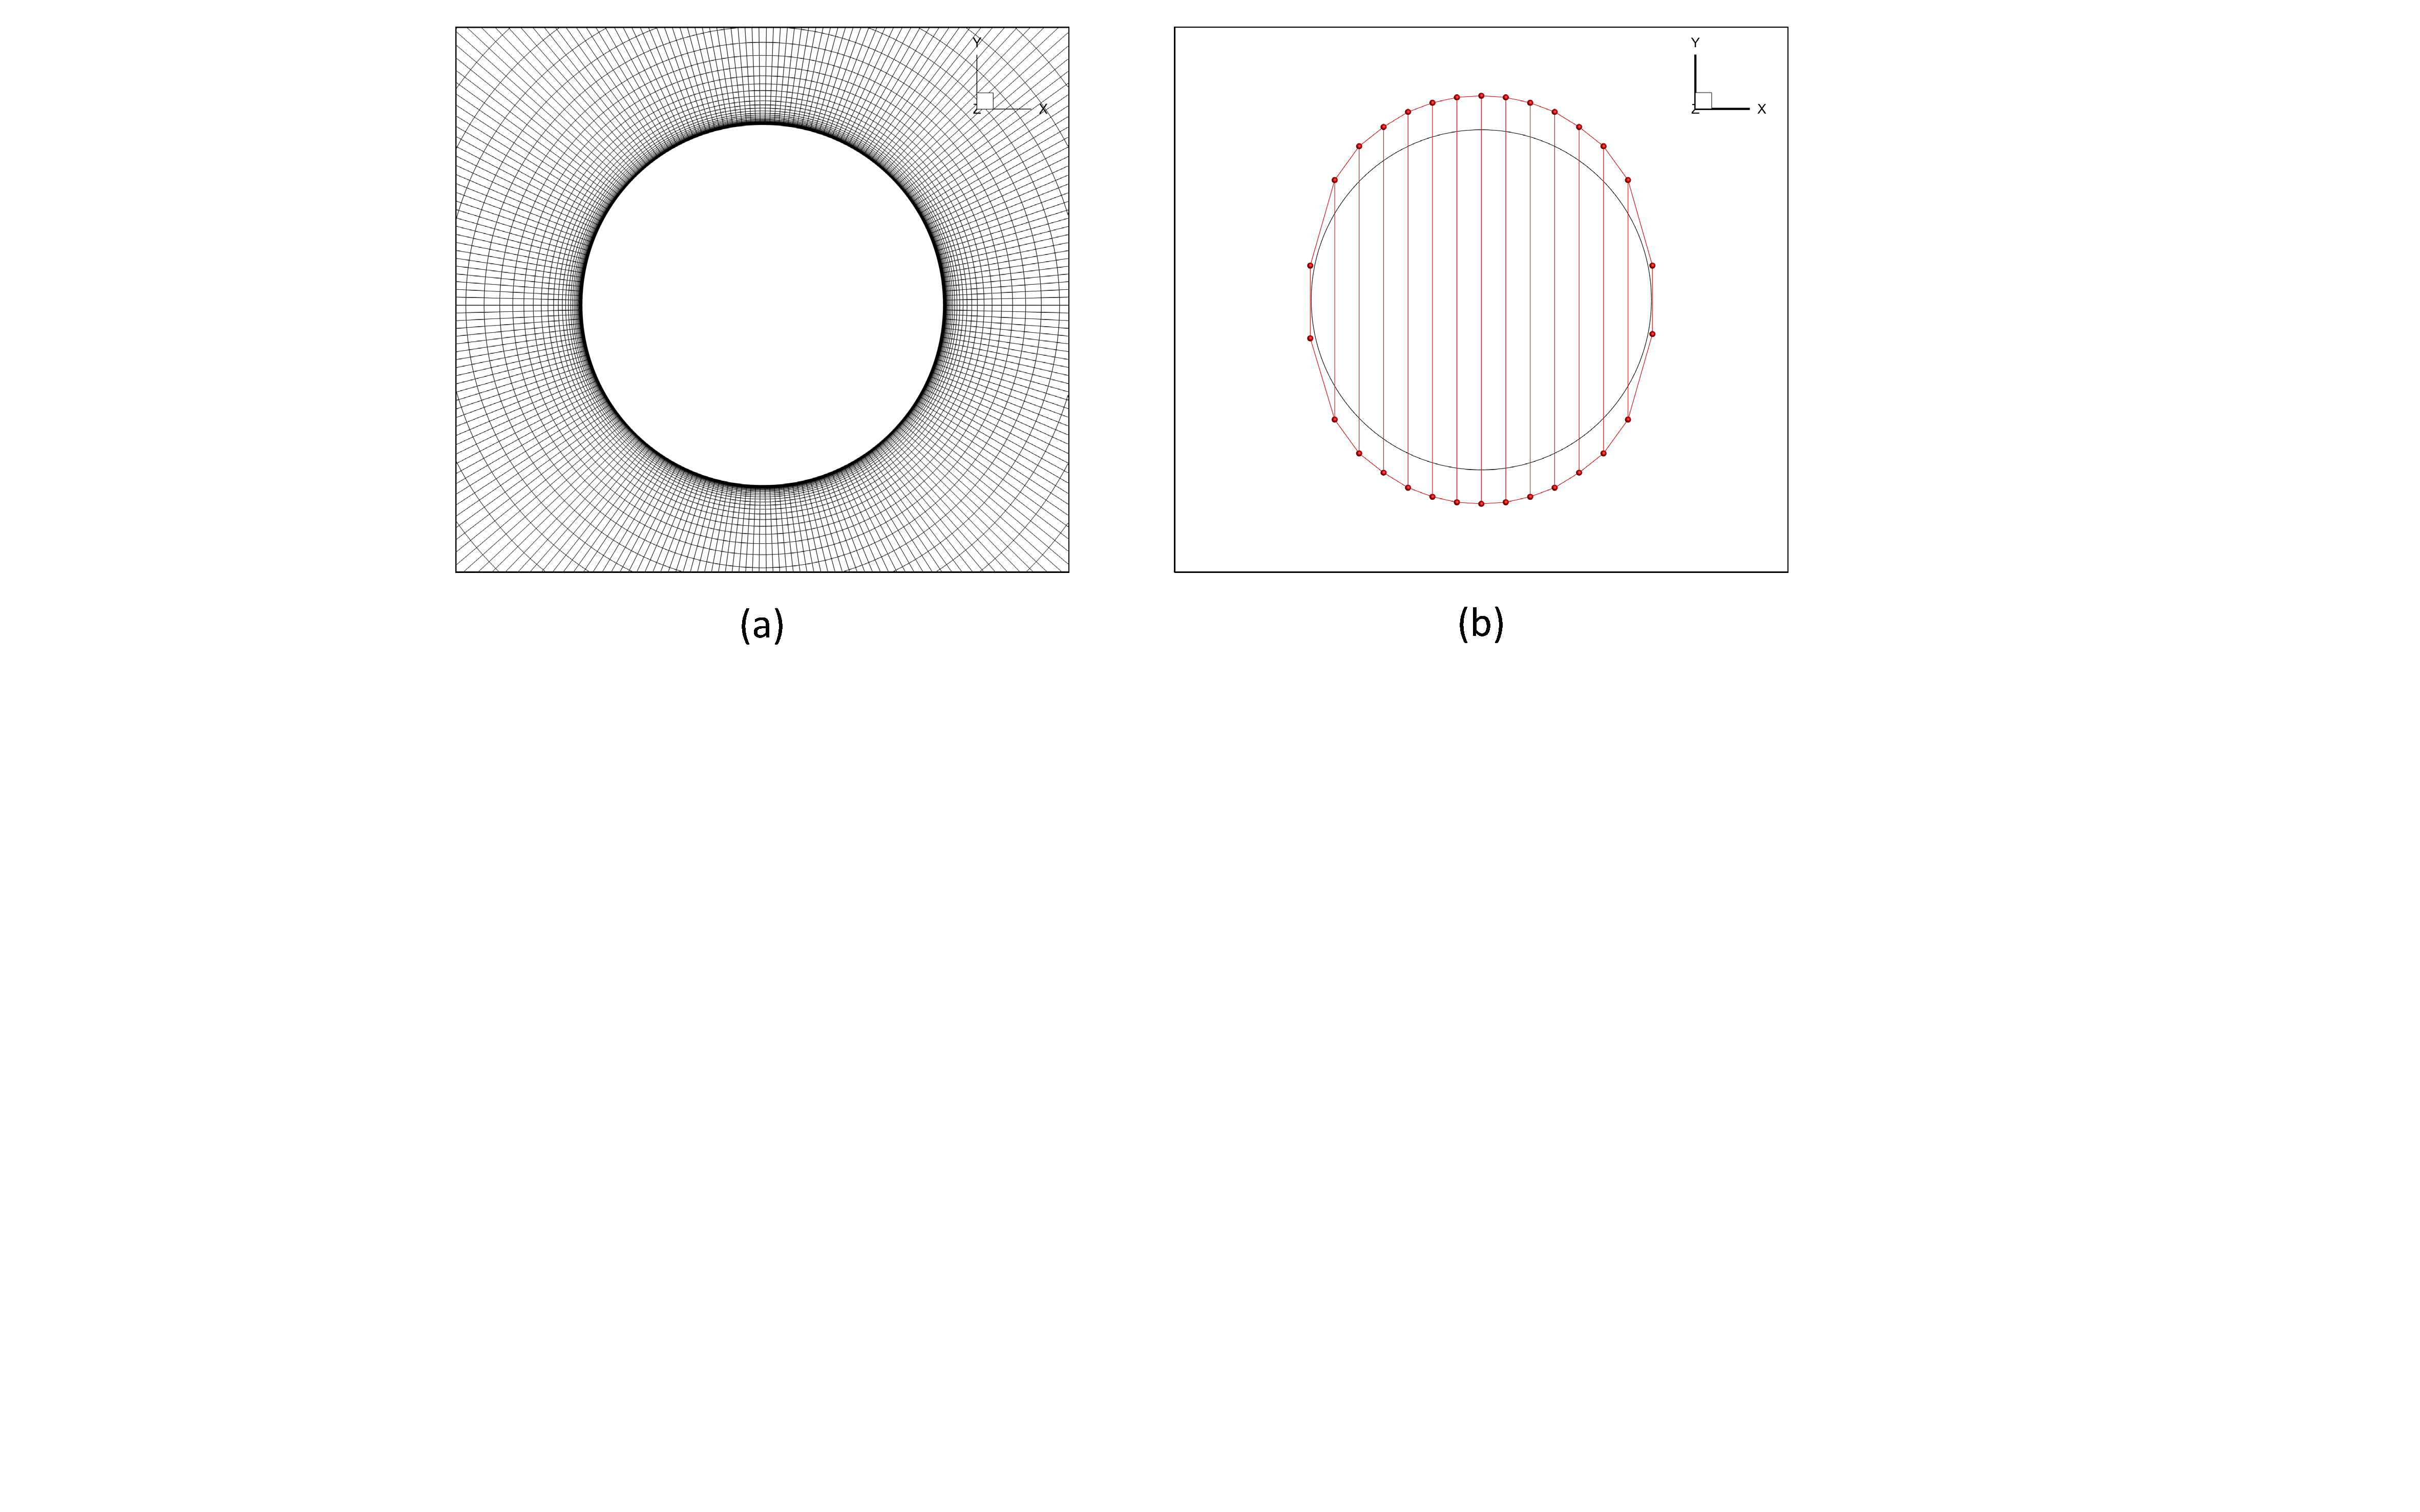
\includegraphics[width=0.8\linewidth]{chapter5/fig/circle2airfoil_template_mesh_initial_geometry.pdf}
    \end{center}
     \vspace{-7mm}
    \caption{
        \small Geometric setup in the 2D airfoil case. (a) DeepGeo template mesh $\hat{M}$. (b) Control points for the FFD baseline.
    }
    \label{ch5:fig:cs1_template_mesh}
\end{figure}

\begin{figure}[htb]
     \begin{center}
         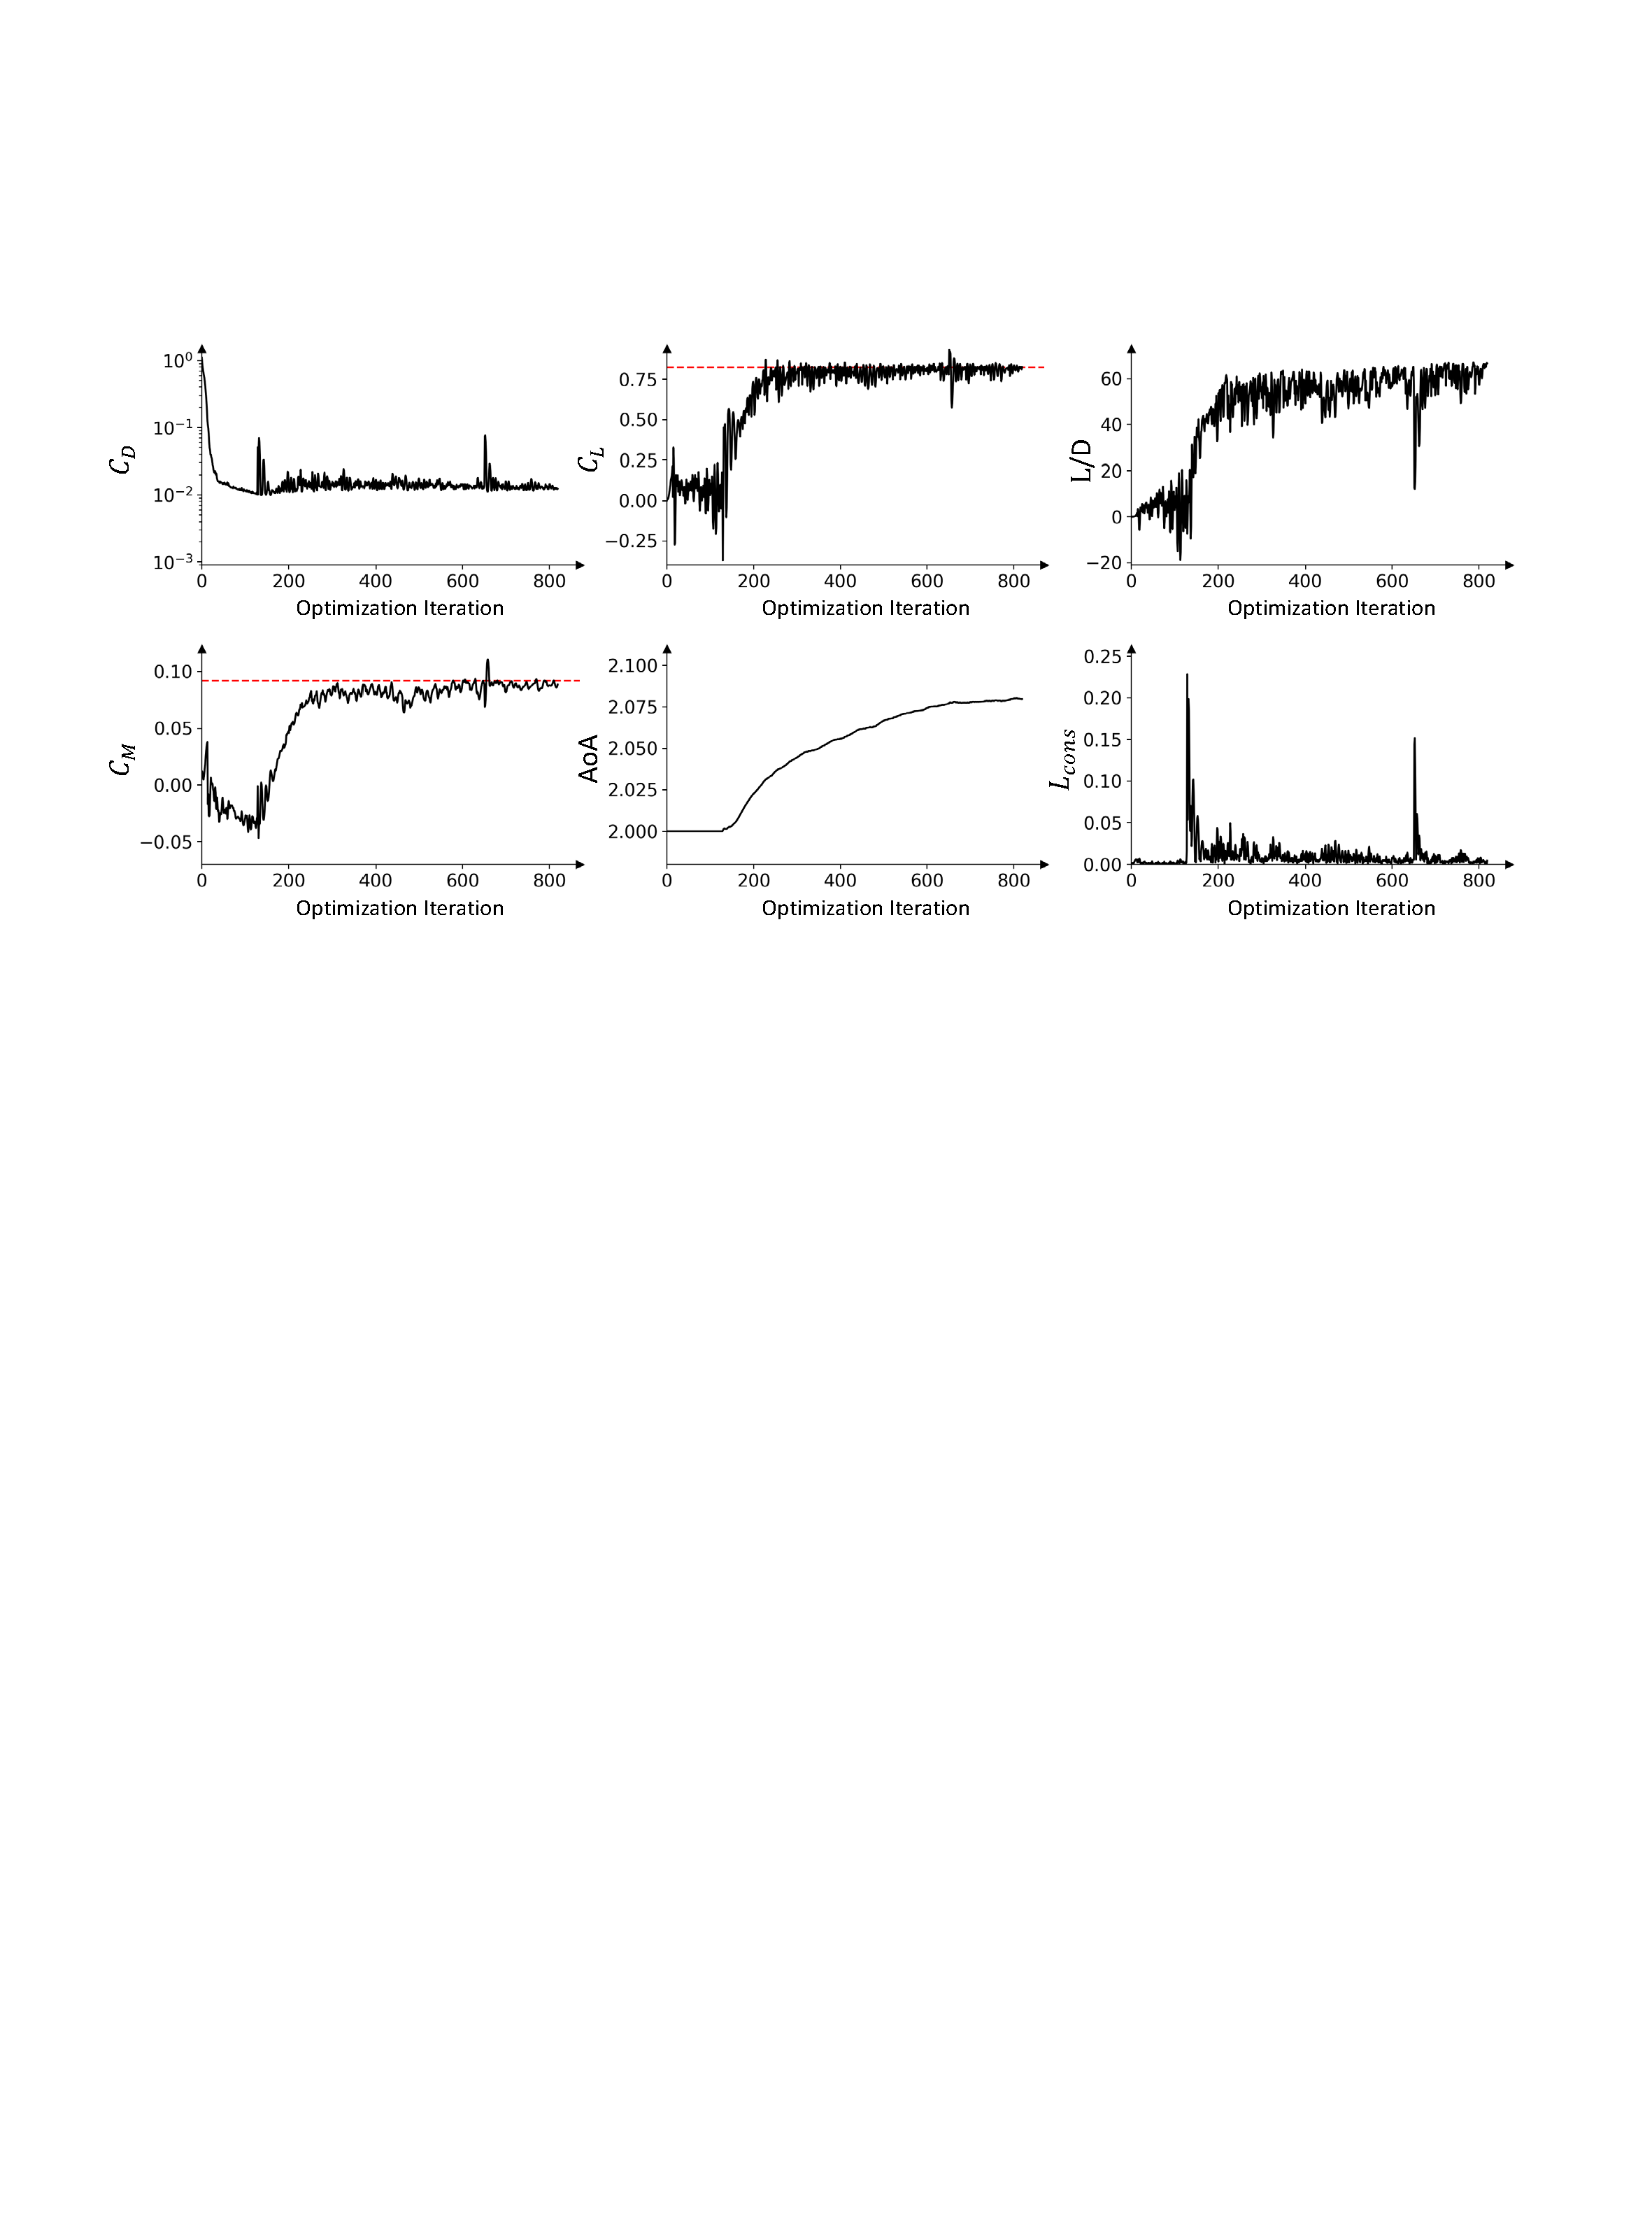
\includegraphics[width=1\linewidth]{chapter5/fig/circle2airfoil_optim_history.pdf}
     \end{center}
      \vspace{-7mm}
     \caption{
         \small Evolution of important quantities during optimization for the 2D airfoil case. The dashed lines in the $C_L$ and $C_M$ plots indicate the target values for these quantities, which are closely approached by the end of the optimization, demonstrating the precision and effectiveness of the DeepGeo model in reaching aerodynamic targets.
     }
     \label{ch5:fig:cs1_history}
 \end{figure}

\begin{figure}[!htb]
    \begin{center}
        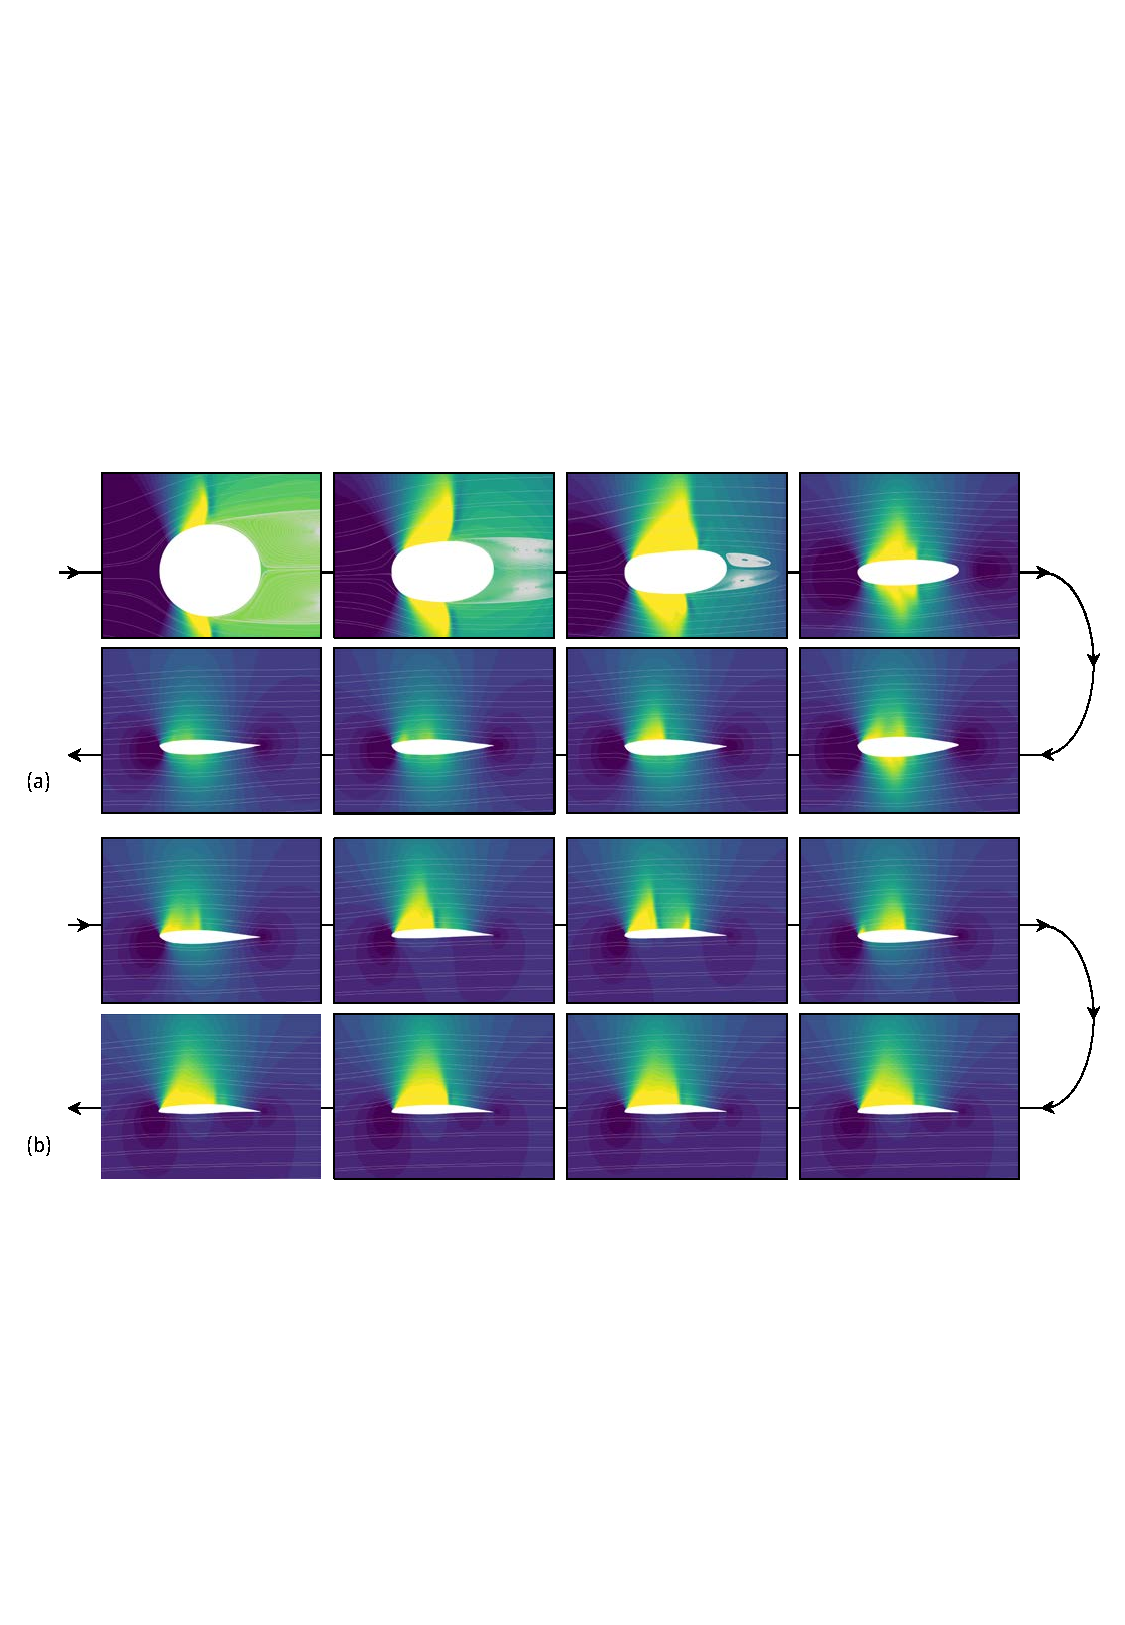
\includegraphics[width=1\linewidth]{chapter5/fig/circle2airfoil_optim_field_visualization.pdf}
    \end{center}
      \vspace{-7mm}
    \caption{
        \small  Evolution of the pressure coefficient field in the 2D airfoil case.  (a) Minimizing $C_D$ alone. (b) Minimizing $C_D$ while setting a target for $C_L$ and $C_M$.
    }
    \label{ch5:fig:cs1_cp}
\end{figure}

\subsubsection{Configuring DeepGeo}

Following the same optimization strategy proposed in~\citet{aa.Li2021}, we perform a two-step optimization. First, the drag coefficient $C_D$ is minimized. Then, terms are added to the objective function to address the lift and moment coefficients, $C_L$ and $C_M$, and the optimization continues. For this purpose, two versions of the function $ \cO_{CFD}$ from Eq.~\ref{ch5:eq:asoObj} are defined to represent the physical objectives as:
%
\begin{align}
    &\cO_{CFD,1} = \left| C_D \right|\;, \\
    &\cO_{CFD,2} = \left| C_D \right| + \left| C_L-0.824 \right| + \max \left( -0.092 - C_M, 0 \right) \;, \nonumber 
\end{align}
%
where the coefficients are obtained with the adjoint solver (denoted as $g$) as $(C_D,C_L,C_M)=g\left(\{\hat{V}+F_\Theta(\hat{V}),E\}\right)$. 
We use the Shoelace formula to compute deformed airfoil's area $A(V^S)$. The geometric loss $\cL_{cons}$ includes a term that constrains the area from falling below the RAE 2822 profile area (\num{0.0654}), along with two additional terms that fix the leading and trailing edge vertices (LE and TE), respectively. This is expressed as:
 %
\begin{equation}
    \cL_{cons} = 
    \underbrace{\max {(0.0654-A(V^S),0)}^2}_\text{area constraint} + 
    \underbrace{\left|\left| \delta\bv^\text{LE} \right|\right|^2}_\text{LE constraint} + 
    \underbrace{\left|\left| \delta\bv^\text{TE} \right|\right|^2}_\text{TE constraint}\;.
\end{equation}
%
As discussed in Section~\ref{ch5:sec:implement}, we use the initial mesh as the template mesh $\hat{M}$.  Tab.~\ref{ch5:tab:circle_2_airfoil_DV_cons} summarizes our experimental setup. 

\begin{figure}[ht]
    \begin{center}
        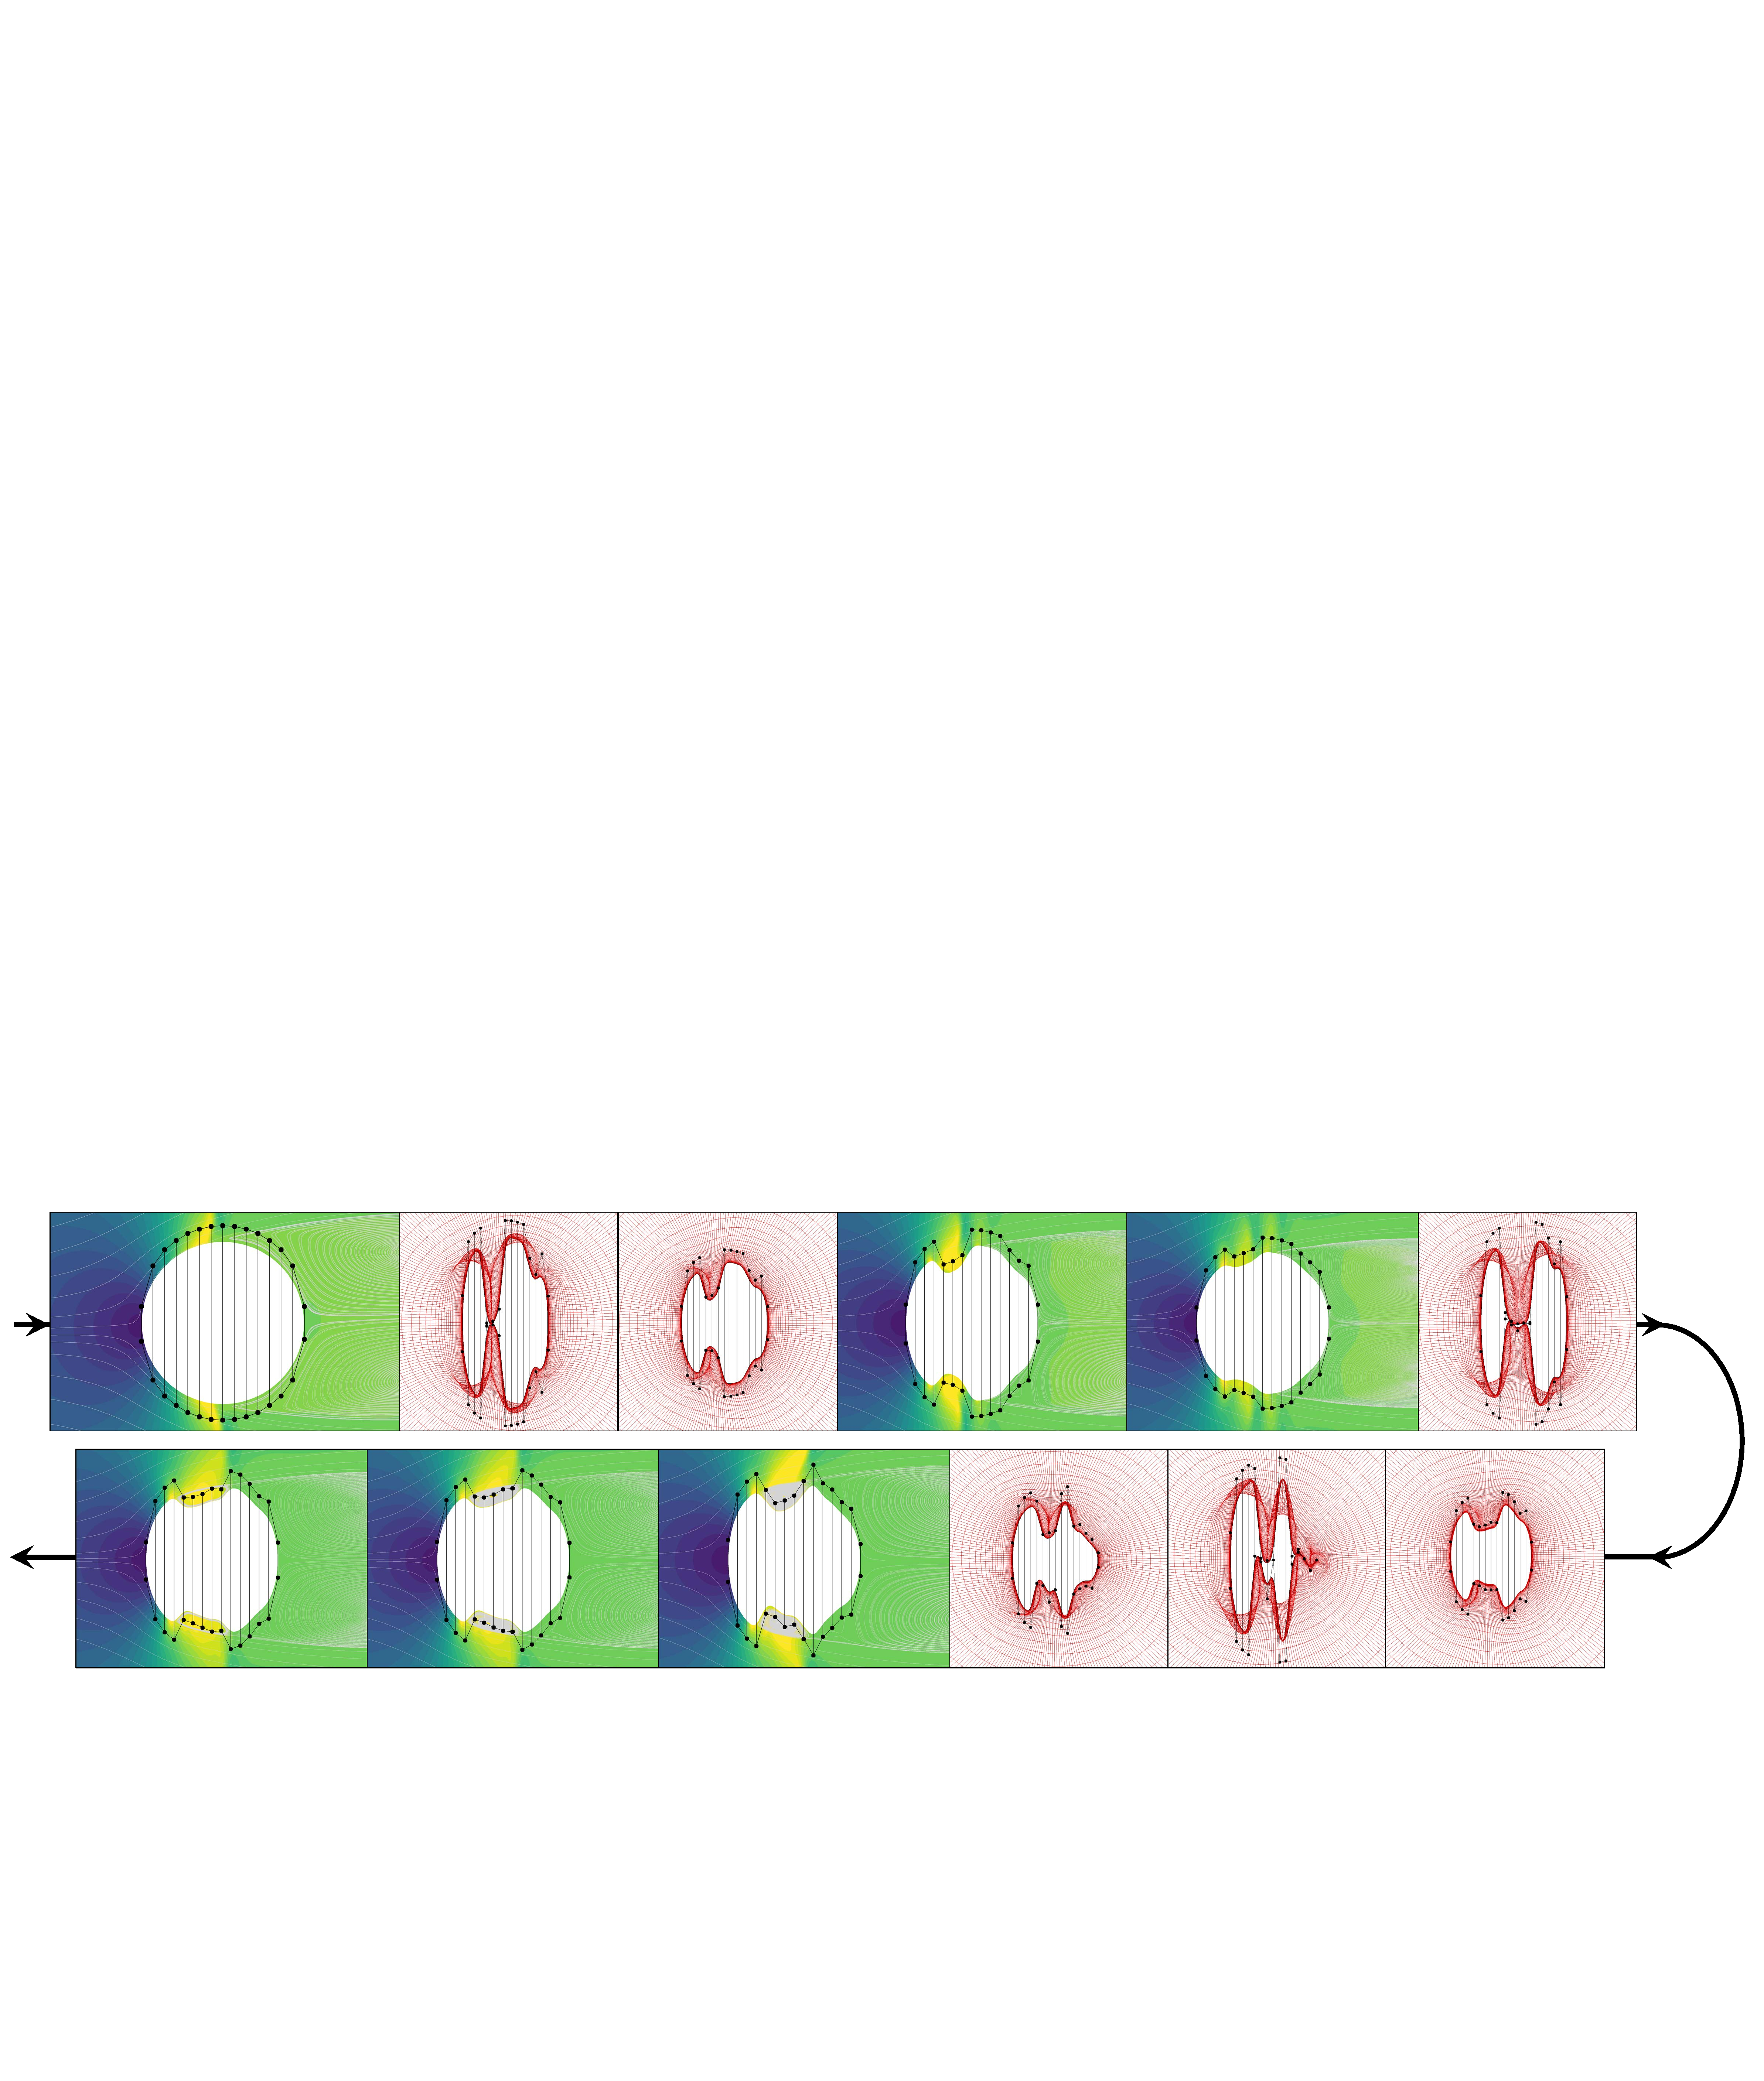
\includegraphics[width=1\linewidth]{chapter5/fig/circle2airfoil_ffd_optim_field_visualization.pdf}
    \end{center}
     \vspace{-7mm}
    \caption{
        \small Failing FFD-based optimization in the 2D airfoil case. The absence of a colored fluid field denotes a simulation that did not converge.
    }
    \label{ch5:fig:cs1_ffd_cp}
\end{figure}

\subsubsection{Configuring the Free-Form Deformation Baseline}

For comparison purposes, we use the implementation of~\cite{aa.Li2021} with a 30-point configuration for FFD as shown in Fig.~\ref{ch5:fig:cs1_template_mesh}(b).
Let the airfoil thickness be $t$, and let $t_\text{RAE2822}$ represent the thickness of the RAE-2822 airfoil.
A set of thickness constraints $t \geq 0.2,t_\text{RAE2822}$ is applied to prevent negative volume errors at the beginning of the optimization. The optimization is conducted using the SLSQP optimizer available in pyOptSparse\cite{aa.Wu2020}.

\subsubsection{Results and Analysis}
\label{ch5:sec:circle_2_airfoil_result}

The optimization process is illustrated in Fig.~\ref{ch5:fig:cs1_history}, while the fluid field changes are visualized in Fig.~\ref{ch5:fig:cs1_cp}. When minimizing $\cO_{CFD,1}$, the drag coefficient $C_D$ is reduced significantly by $99.1\%$.
The shape gradually and smoothly becomes thinner, with the leading and trailing edges emerged and symmetry largely preserved. No singular shapes or simulation failures occur, demonstrating the robustness of DeepGeo to large mesh deformations.
In the second stage, symmetry is broken to achieve a streamlined profile commonly observed in high-lift transonic airfoils, effectively generating more lift.
A shock wave initially appears but is gradually diffused, and by the end of the optimization, it largely dissipates.
The final airfoil achieves  $C_D=\num{0.012195}$ (i.e. $121.95$ counts), and its lift-over-drag ratio ($L/D$) is significantly improved from \num{1e-3} to $67.22$, which makes it  comparable to that of modern supercritical airfoils designed for transonic flights. This result validates DeepGeo’s effectiveness in achieving high-performance designs.

In contrast, the FFD-based optimization fails after a small number of iterations due to singularities in the deformed shape, leading to severe meshing issues as shown in Fig.~\ref{ch5:fig:cs1_ffd_cp}. In some iterations, simulation failure occurs, represented by the mesh in red. 
Although FFD ensures local smoothness within a control cage, the free movement of control points can lead to global singularities and geometric abnormalities. These issues persist despite adjustments to the hyperparameters. Such failures do not occur with DeepGeo, highlighting its stability and reliability for complex shape optimizations that require high deformation freedom. 